\solution 
Points $\vec{A},\vec{D},\vec{G}$ are defined to be collinear if 
\begin{align}
    \text{rank}\myvec{
    1 & 1 & 1\\
    \vec{A} & \vec{D} & \vec{G} \\
    } = 2 
    \label{eq:mat_row_operations}
    \\
\implies    
    \myvec{
    1 & 1 & 1
    \\
    1 & -\frac{7}{2} & -2
    \\
    -1 & \frac{1}{2} & 0
    }
     \xleftrightarrow[]{R_3 \leftarrow R_3+R_2}
    \myvec{
    1 & 1 & 1
    \\
    1 & -\frac{7}{2} & -2
    \\
    0 & -3 & -2 
    }
    \\
     \xleftrightarrow[]{R_2\leftarrow R_2-R_1}
    \myvec{
    1 & 1 & 1
    \\
    0 & -\frac{9}{2} & -3
    \\
    0 & -3 & -2 
    }
     \xleftrightarrow[]{R_3\leftarrow R_3-\frac{2}{3}R_2}
    \myvec{
    1 & 1 & 1
    \\
    0 & -\frac{9}{2} & -3
    \\
    0 & 0 & 0
    }
\end{align}
Thus, the matrix 
    \eqref{eq:mat_row_operations}
    has rank 2 and the points are collinear.
    Thus, the medians of a triangle meet at the point $\vec{G}$.
See \figref{fig:Triangle-median}.
\begin{figure}
\centering
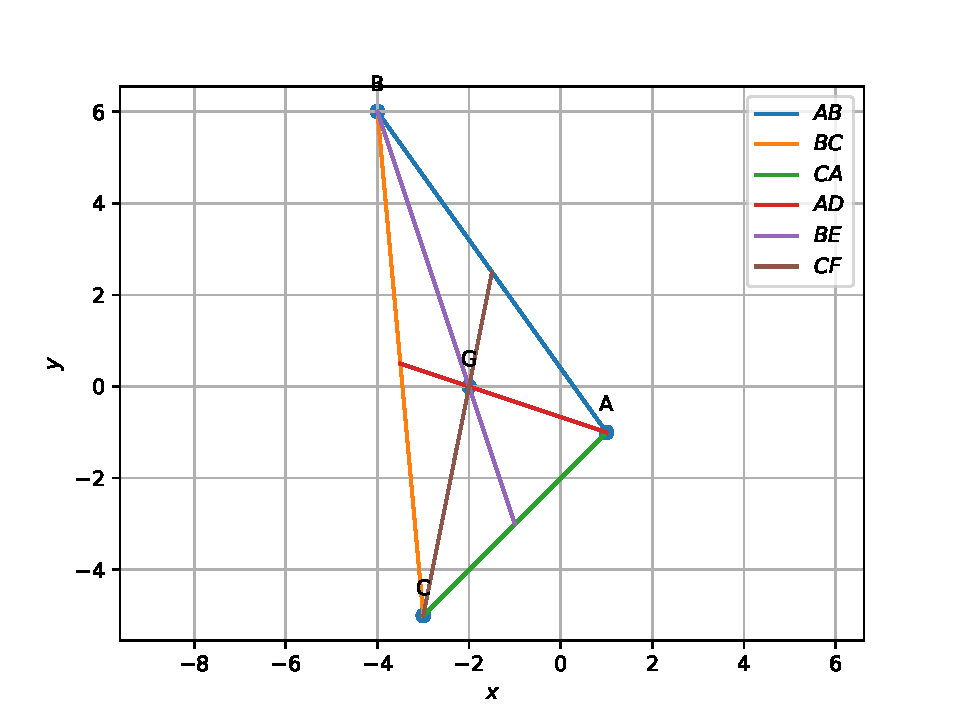
\includegraphics[width=0.75\columnwidth]{figs/triangle/median.pdf}
	\caption{Medians of $\triangle ABC$ meet at $\vec{G}$.}
\label{fig:Triangle-median}
\end{figure}

